\setcounter{section}{4} % This causes the next section to be Appendix B


\section*{Examples IV. 3D Time-dependent Behavior Examples}
\label{PS4}

This set of example problems is due on November 17, 2025. 

\medskip
\subsection*{4--1. \textbf{Characterization with deflection history} [4 pts].} 
A simply supported beam \textcolor{red}{with a uniform applied load (or you could instead use a point end load on a cantilevered beam as I mentioned on Slack, either is completely fine)} is made from a material that is well-described by a three-parameter standard linear solid model, i.e., the general creep compliance function $J_c(t)$ is given by
\begin{equation*}
    J_c(t) = J_\infty + (J_0 - J_\infty) \exp\left[-\frac{t}{\tau_c}\right],
\end{equation*}
where $J_\infty$, $J_0$, and $\tau_c$ are all mechanical properties of the material. 

The beam has a length of 4 ft and a second moment of area about the out-of-plane axis of 1 in$^4$. 
It is subjected to a position-time separable load function $q(z,t) = \hat{q}(z) \phi(t)$ where $\phi(t) = -3$ lb/ft $\cdot \mathcal{H}(t)$. 
Say we determine the maximum deflection in the beam at different times to be
\begin{align}
    &u_y \Big|_{\max} = -0.6 \textrm{~in~~at~~}t=30\textrm{~min}\\
    &u_y \Big|_{\max} = -0.75 \textrm{~in~at~~}t=60\textrm{~min}\\
    &u_y \Big|_{\max} = -1.0 \textrm{~in~~at~~}\textrm{~long times}
    \end{align}
From this, calibrate the material properties.

\bigskip
\textit{Solution.}

I will begin by solving the linear elastic problem for the point load cantilever with a force of 12 lb at the end of the beam. From a quick shear-force bending moment diagram of the beam, we can determine that $\hat{M}_x(z) = 12(L-z)$

\begin{align*}
    \frac{d^2u_y(z)}{dz^2} &= \frac{\hat{M}_x(z)}{EI_x} \\
    &= \frac{12(L-z)}{EI_x} \\
    &= \frac{12(L-z)}{E(1)} \\
    &= \frac{12(z-L)}{E} \\
\end{align*}
Integrating yields
\begin{align*}
    \frac{du_y(z)}{dz} &= \int\frac{12(z-L)}{E} dz\\
    &= \frac{12}{E}\left( \frac{1}{2}z^2-Lz + C_1 \right) \\
    u_y(z) &= \int\frac{12}{E}\left( \frac{1}{2}z^2-Lz + C_1 \right) dz \\
    &= \frac{12}{E}\left(\frac{1}{6}z^3-\frac{L}{2}z^2+C_1z+C_2 \right) \\
\end{align*}
Applying the known boundary conditions that $u_y(0) = 0$ and $u_y'(0) = 0$ we see that both integration constants are themselves equal to 0 yielding an elastic solution of
\begin{align*}
    u_y(z) &= \frac{12}{E}\left(\frac{1}{6}z^3-\frac{L}{2}z^2\right) \\
    u_y\Big|_{\max} &= u_y(L) \\
    &= \frac{12}{E} \left( -\frac{L^3}{3} \right)\\
    &= -\frac{4L^3}{E} \\
    u_y\Big|_{\max}(t) & = -\frac{4L^3}{E_c(t)} \\
    & = -\frac{4*(4*12)^3}{E_c(t)} \\
    & = -\frac{442368}{E_c(t)} \text{ [($E_c(t)$ has units of lb/in$^2$}]\\
    &= -442368J_c(t) \text{ [($J_c(t)$ has units of in$^2$/lb}] \\
\end{align*}

Note that here a formal convolution was not needed because of the step function loading condition. Had $\phi(t)$ been time-varying within our convolution integral bounds of $0^-$ to $t$ then we would have had to used Laplace transforms to solve the integral. Now we can solve for the constants of $J_c(t)$ 

\begin{align*}
    u_y\Big|_{\max}(\infty) &= -442368 J_c(\infty) \\
    -1 &= -442368J_\infty \\
    \therefore J_\infty &= \frac{1}{442368} \\
    &= 2.261\times 10^{-6} \text{ in$^2$/lb}
\end{align*}

Solving the remaining system of equations from the two other known deflection states we can see that 
\begin{align*}
    \tau_c  &= 63.8\text{ min} \\
    J_0 &= 5.083\times 10^{-7}\text{ in$^2$/lb}
\end{align*}


\bigskip
\subsection*{4--2. \textbf{Ramp up the torque} [4 pts].} 
A viscoelastic cylinder $AB$ is fixed on its end $A$ and simply supported on its opposite end at $B$. 
At point $B$, a second, rigid rod is joined to the end such that exerting a force on the rod will induce a counterclockwise torque about the axis of $AB$. 
A point force of magnitude $P_0$ is applied to the rigid rod, causing the front face to turn counterclockwise. 
The point force travels along the rod such that its distance from the bar's neutral axis $a(t)$ is direct in time, i.e., $a(t) = \alpha t$, where $\alpha$ is a constant. 
What is the angular rotation of the end $B$ as a function of time, $\Phi(t)$?

\bigskip
\textit{Solution.}

I begin by solving for the elastic solution for the angular rotation of the end of B.

\begin{align*}
    \Phi &= \frac{TL}{\mu J} \\
    &= \frac{(P_0\alpha t)L}{\mu (\pi R^4/2)} \\
    &= \frac{2P_0\alpha L}{\pi \mu R^4} t\\
\end{align*}

For the viscoelastic case we apply the correspondence principle.

\begin{align*}
    \Phi(t) &= \frac{L}{J}\int_{0^-}^t \mu_c(t-\tau)\frac{d(P_0\alpha \tau)}{d\tau}d\tau \\
    &= \frac{L}{\pi R^4/2}\int_{0^-}^t \mu_c(t-\tau)(P_0\alpha) d\tau \\
    &= \frac{2P_0\alpha L}{\pi R^4}\int_{0^-}^t \mu_c(t-\tau) d\tau \\
\end{align*}

\bigskip
\subsection*{4--3. \textbf{L-shaped beam} [4 pts].}
\begin{wrapfigure}[8]{r}{2in}
\vspace{-1cm}
    \centering
     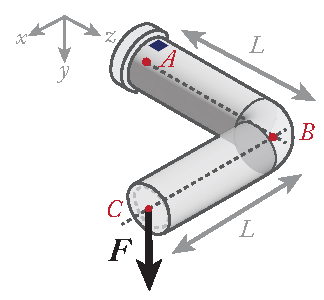
\includegraphics[scale=1]{instr-figures/L-bracket.pdf}
    \caption*{Figure 4.3a.}
    \label{fig:Lbracket}
\end{wrapfigure}
A one-piece polymeric member \textit{ABC} consists of two segments of length $L$ at a right angle from one-another and encastred at $A$, as shown. 
Its neutral axes both lie in the $x-z$ plane when unloaded. 
Assuming the creep compliance in shear to be $\mu_c(t)$ and the creep compliance in axial tension to be $E_c(t)$, determine (a) the deflection at $C$ in terms of the time-varying force $F(t)$ and (b) the stress tensor $\mathbf{\sigma}(t)$ at the square surface element located above $A$.  

\bigskip
\textit{Solution.}

I begin by solving the elastic solution for the beam. One can see that the shear stress will be -F throughout the length of AB and BC. This will yield two separate, but equal contributions to the deflection at C from bending of each section due to AB and BC having the same length. The torsional displacement about the z-axis in AB contributes a third term to the deflection expression.

\begin{align*}
    u_z(C) &= 2\left( \frac{FL^3}{3EI}\right) + L\left(\frac{M_z(B)L}{\mu J}\right) \\
    &= \frac{2FL^3}{3EI} + \frac{FL^3}{\mu J} \\
    &= \frac{2FL^3}{3E(\pi R^4/4)} + \frac{FL^3}{\mu (\pi R^4/2)} \\
    &= \frac{8FL^3}{3\pi E R^4} + \frac{2FL^3}{ \pi \mu R^4} \\
\end{align*}

To applying correspondence principle:

\begin{align*}
     u_z(C,t) &=\int_{0^-}^t  \left( \frac{8L^3}{3\pi R^4}E_c(t-\tau) + \frac{2L^3}{\pi R^4}\mu_c(t-\tau) \right) \frac{dF(\tau)}{d\tau}d\tau \\
     &= \frac{8L^3}{3\pi R^4}E_c*\dot{F} + \frac{2L^3}{\pi R^4}\mu_c*\dot{F} \qed \\
\end{align*}

For part (b), we will now find the stress tensor for region A on the figure. Note that the region is in the x-z plane at the top of the bar so the shear stresses in AB in the y-direction will not contribute. There will be an axial contribution in the z-direction from the bending that will be positive because of the orientation of the bending. There will also be an x-z shear component from the torsion in AB.

{ \allowdisplaybreaks \begin{align*}
        \sigma_{xz} &= \sigma_{zx} \\
        &= \frac{Tr}{J} \\
        &= \frac{FLR}{(\pi R^4/2)} \\
        &= \frac{2FL}{\pi R^3} \\
        \sigma_{zz} &= \frac{MR}{I} \\
        &= \frac{(FL)R}{\pi R^4/4} \\
        &= \frac{4FL}{\pi R^3} \\
        \sigma(A) &=  \begin{bmatrix}
        0 & 0 & \sigma_{xz} \\ 0 & 0 & 0 \\ \sigma_{zx} & 0 & \sigma_{zz} \end{bmatrix} \\
\end{align*}}

Now we apply correspondence once again to get the time-dependent form of this solution:

\begin{align*}
    \sigma_{xz}(A,t) &= \sigma_{zx}(A,t) \\
    &= \int_{0^-}^t 2 \mu_r(t-\tau)\frac{d\varepsilon_{zx}(\tau)}{d\tau}d\tau \\
    &= \int_{0^-}^t2\mu_r(t-\tau)\frac{2L}{\pi R^3}\frac{dF(\tau)}{d\tau}d\tau \\
    &= \frac{4L}{\pi R^3} \int_{0^-}^t\mu_r(t-\tau)\frac{dF(\tau)}{d\tau}d\tau \\
    &= \frac{4L}{\pi R^3} \mu_r * \dot{F}\\
    \sigma_{zz}(A,t) &= \int_{0^-}^t E_r(t-\tau)\frac{d\varepsilon_{zz}(\tau)}{d\tau}d\tau \\
    &= \int_{0^-}^t E_r(t-\tau)\frac{4L}{\pi R^3}\frac{dF(\tau)}{d\tau}d\tau \\
    &= \frac{4L}{\pi R^3}\int_{0^-}^t E_r(t-\tau)\frac{dF(\tau)}{d\tau}d\tau \\
    &= \frac{4L}{\pi R^3} E_r * \dot{F} \\
    \sigma(A,t) &=  \begin{bmatrix}
        0 & 0 & \sigma_{xz}(A,t) \\ 0 & 0 & 0 \\ \sigma_{zx}(A,t) & 0 & \sigma_{zz}(A,t) \end{bmatrix} \\
\end{align*}


\newpage
\subsection*{4--4. \textbf{Fibrous material} [4 pts].}
An elastic material with a fiber phase has the Helmholtz free energy function
\begin{equation*}
\widetilde{\psi}(\bn{F}) = \frac{1}{2}C_{10} (I_1-3) + \frac{1}{4} k (I_a - 1)^2,
\end{equation*}
where $I_1(\bn{C}) = \textrm{tr}(\bn{C})$ and $I_a(\bn{C},\hat{\bm{a}}_0) = \hat{\bm{a}}_0 \cdot \bn{C} \hat{\bm{a}}_0$ for $\bn{C} = \bn{F}^\intercal \bn{F}$.

%\skiponeline
%(a) Show that, given the direction $\hat{\bm{a}}_0$ is fixed by the material, $I_a$ is an invariant of $\bn{C}$.

\medskip
(a) Show that this elastic potential is consistent with the principle of objectivity.

\bigskip
\textit{Solution.}

$\widetilde{\psi}$ is said to be objective if and only if $ \widetilde{\psi}(\bn{F}) = \widetilde{\psi}(\bn{QF})$ where $\bn{Q}$ is a an arbitrary proper orthogonal tensor acting as a rigid body rotation on our deformation gradient tensor $\bn{F}$. For convenience, I will denote $\bn{QF}$ as $\bn{F}^*$. Of the values in the function, only $I_1$ and $I_a$ are functions of $\bn{C} = \bn{C}(\bn{F})$ within the elastic potential function. If $\bn{C}$ is objective, then  $I_1$ and $I_a$ are objective which implies that $\widetilde{\psi}$ is as well. First I will check whether $I_1$ is objective. 

\begin{align*}
    \bn{C} &= \bn{F}^T\bn{F} \\
    \bn{C}^* &= (\bn{F}^*)^T\bn{F}^* \\
    &= (\bn{QF})^T\bn{QF} \\
    &= \bn{F}^T\bn{Q}^T\bn{QF} \\
    &= \bn{F}^T\bn{F} \\
    &= \bn{C} \\
    \therefore I_1(\bn{C}) = I_1(\bn{C}^*) \\
    \therefore I_a(\bn{C}) = I_a(\bn{C}^*)
\end{align*} 

All terms in $\widetilde{\psi}$ have been proven to be objective, therefore the elastic potential itself must be objective as well, or more formally $\widetilde{\psi}(\bn{F}) = \widetilde{\psi}(\bn{F}^*)$

\medskip
(b) Show that the material symmetry group $\mathcal{G}$ is the set of all proper orthogonal tensors $\bn{H}$ with $\bn{H}\hat{\bm{a}}_0 = \hat{\bm{a}}_0$.  

To prove the symmetry condition, we must prove that $I_a(\bn{C},\hat{\bm{a}}_0)$ is equal to a rotated system $I_a(\bn{H}\bn{C}\bn{H}^T,\bn{H}\hat{\bm{a}}_0)$ if and only if $\bn{H}\hat{\bm{a}}_0 = \hat{\bm{a}}_0$. The $I_1$ term in is not discussed here because the trace of a tensor invariant under rotation.

\begin{align*}
    I_a(\bn{C},\hat{\bm{a}}_0) &= \hat{\bm{a}}_0 \cdot \bn{C} \hat{\bm{a}}_0 \\
    &= \hat{\bm{a}}_0^T \bn{C} \hat{\bm{a}}_0 \\
    I_a(\bn{H}\bn{C}\bn{H}^T,\bn{H}\hat{\bm{a}}_0) &= (\bn{H}\hat{\bm{a}}_0)^T\bn{HCH}^T(\bn{H}\hat{\bm{a}}_0) \\
    &= \hat{\bm{a}}_0^T\bn{H}^T\bn{HCH}^T\bn{H}\hat{\bm{a}}_0 \\
    &= \hat{\bm{a}}_0^T\bn{C}\hat{\bm{a}}_0 \\
    \therefore I_a(\bn{C},\hat{\bm{a}}_0) &= I_a(\bn{H}\bn{C}\bn{H}^T,\bn{H}\hat{\bm{a}}_0)
\end{align*}

The $I_a$ term is equivalent if and only if both the reference frame for the right Cauchy-Green tensor \textit{and} the fiber direction are both rotated in the same manner. If we rotated our basis for the strains and then had any proper orthogonal rotation, $\bn{Q} \neq \bn{H}$, applied to our fiber direction (i.e., $I_a(\bn{HCH}^T,\bn{Q}\hat{\bm{a}}_0)$), then the terms would be different outside the trivial case of isotropy where properties are independent of fiber direction.

\medskip
(c) Find the first Piola-Kirchhoff and Cauchy stress expressions with an applied deformation gradient tensor of $\bn{F}$.

\bigskip
\textit{Solution.}
{ \allowdisplaybreaks \begin{align*}
    \bn{P} &= \frac{\partial\widetilde{\psi}}{\partial\bn{F}} \\
    &= \frac{\partial\widetilde{\psi}}{\partial I_1}\frac{\partial I_1}{\partial\bn{F}} + \frac{\partial\widetilde{\psi}}{\partial I_a}\frac{\partial I_a}{\partial\bn{F}} \\
    \frac{\partial\widetilde{\psi}}{\partial I_1} &= \frac{C_{10}}{2} \\
    \frac{\partial\widetilde{\psi}}{\partial I_a} &= \frac{k}{2}(I_a - 1) \\
    \frac{\partial I_1}{\partial F_{mn}} &= \frac{\partial\textrm{tr}(F_{ji}F_{jk})}{F_{mn}} \\
    &= \frac{\partial F_{ji}F_{ji}}{F_{mn}} \\
    &= 2 \frac{\partial F_{ji}}{\partial F_{mn}} F_{ji} \\
    &= 2\delta_{jm}\delta_{in}F_{ji} \\
    &= 2F_{mn} \\
    \implies \frac{\partial I_1}{\partial \bn{F}} &= 2\bn{F} \\
    \frac{\partial I_a}{\partial F_{mn}} &= \frac{\partial(\hat{\bm{a}}_0)_i F_{ki}F_{kj}(\hat{\bm{a}}_0)_j}{\partial F_{mn}} \\
    &= (\hat{\bm{a}}_0)_i (\hat{\bm{a}}_0)_j (\delta_{km}\delta_{in}F_{kj} + F_{ki}\delta_{mk}\delta_{jn}) //
    &= (\hat{\bm{a}}_0)_n (\hat{\bm{a}}_0)_j F_{mj} + (\hat{\bm{a}}_0)_i (\hat{\bm{a}}_0)_n F_{mi} \\
    &= 2 F_{mn} (\hat{\bm{a}}_0)_n (\hat{\bm{a}}_0)_j \\
    \implies \frac{\partial I_a}{\partial \bn{F}} &= 2(\bn{F}\hat{\bm{a}}_0) \otimes \hat{\bm{a}}_0 \\
    \therefore \bn{P} &= C_{10}\bn{F} + k(I_a-1)(\bn{F}\hat{\bm{a}}_0)\otimes \hat{\bm{a}}_0
\end{align*}}

Using a push-forward operation to calculate for the Cauchy stress: 

\begin{align*}
    \bm{\sigma} &= J^{-1} \bn{PF}^T \\
    &= J^{-1}(C_{10}\bn{FF}^T + k(I_a-1)(\bn{F}\hat{\bm{a}}_0)\otimes \hat{\bm{a}}_0 \bn{F}^T) \\
    &= \frac{1}{\textrm{det}\bn{F}} (C_{10}\bn{B} + k(I_a-1)(\bn{F}\hat{\bm{a}}_0)\otimes(\bn{F}\hat{\bm{a}}_0))  \\
\end{align*}

\bigskip
\bigskip
\subsection*{4--5. \textbf{Gent model of rubber elasticity} [4 pts].}
The Gent model, which incorporates the finite extensibility of polymer chains in a rubber network but includes $I_2$-dependence, has a\textcolor{red}{n isochoric} free-energy function of $$\bar{\Psi}_{\textcolor{red}{\textrm{iso}}} = -\frac{C_{10}}{2} J_m \ln \left(1 - \frac{I_1-3}{J_m} \right) + C_{01}\ln \left(\frac{I_2}{3}\right), $$ where $C_{10}>0$, $C_{01}\geq 0$, and $J_m>0$ are material constants.

\medskip
(a) Show that the Cauchy stress corresponding to the free energy above has the form\footnote{\textcolor{red}{You may want to use the Cayley-Hamilton theorem to do a replacement for $\bn{B}^2$, which produces $\bn{B}^2 = I_1 \bn{B} - I_2 \bn{I} + I_3 \bn{B}^{-1}$.}} $$\bm{\sigma} = -p \bn{I} + \frac{C_{10} J_m}{J_m - (I_1-3)}\bn{B} - \frac{2C_{01}}{I_2} \bn{B}^{-1}.$$

\bigskip
\textit{Solution.}\\

From the course notes, we derived the expression 

\begin{equation*}
    \bn{P} = 2\left( \frac{\partial\Psi}{\partial I_1}-I_1\frac{\partial\Psi}{\partial I_2}\right)\bn{F} - 2\frac{\partial\Psi}{\partial I_2}\bn{BF} + 2I_3\frac{\partial\Psi}{\partial I_3} \bn{F}^{-T}
\end{equation*}

To obtain the Cauchy stress we push $\bn{P}$ forward as follows

\begin{align*}
    \bn{\sigma} &= J^{-1}\bn{PF}^T \\
    &= J^{-1}\left( 2\left( \frac{\partial\Psi}{\partial I_1}-I_1\frac{\partial\Psi}{\partial I_2}\right)\bn{B} - 2\frac{\partial\Psi}{\partial I_2}\bn{B}^2 + 2I_3\frac{\partial\Psi}{\partial I_3} \right)
\end{align*}

Next we convert to a form compatible with an isochoric strain energy density function.

\begin{align*}
    \bm{\sigma} &=  -\bar{p}\bn{I} + 2\left( \frac{\partial\Psi_{iso}}{\partial I_1}-I_1\frac{\partial\Psi_{iso}}{\partial I_2}\right)\bn{B} - 2\frac{\partial\Psi_{iso}}{\partial \bar{I_2}}\bn{B}^2 + 2I_3\frac{\partial\Psi_{iso}}{\partial I_3} \\
\end{align*}

Calculating the derivatives of $\Psi_{iso}$ with respect to the invariants yields: 
\begin{align*}
    \frac{\partial\Psi_{iso}}{\partial I_1} &= \frac{-C_{10}}{2}J_m\frac{1}{1-\frac{1_1-3}{J_m}}\frac{-1}{J_m} \\
    &= \frac{C_{10}}{2}\frac{J_m}{J_m-I_1+3} \\
    \frac{\partial\Psi_{iso}}{\partial I_2} &= C_{01}\frac{1}{I_2/3}\frac{1}{3}  \\
    &= \frac{C_{01}}{I_2} \\
    \frac{\partial\Psi_{iso}}{\partial I_3} &= 0 \\
\end{align*}

Substituting into the Cauchy stress equation, using the provided Cayley-Hamilton theorem to simplify the $\bn{B}^2$ term, and then using $I_3 = 1$ because all terms besides the first are isochoric: 

\begin{align*}
    \bm{\sigma} &= -\bar{p}\bn{I} + 2\left( \frac{C_{10}}{2}\frac{J_m}{J_m-I_1+3} + \frac{I_1 C_{01}}{I_2} \right) \bn{B} - \frac{2 C_{01}}{I_2}(I_1\bn{B} - I_2\bn{I} + I_3\bn{B}^{-1}) \\
    &= -\bar{p}\bn{I} + \frac{C_{10}J_m}{J_m-I_1+3}\bn{B} - \frac{2 C_{01}}{I_2}(- I_2\bn{I} + \bn{B}^{-1}) \\
    &= -\bar{p}\bn{I} + \frac{C_{10}J_m}{J_m-I_1+3}\bn{B} + 2 C_{01}\bn{I} - \frac{2C_{01}}{I_2}\bn{B}^{-1} \\
    &= -p\bn{I} + \frac{C_{10}J_m}{J_m-I_1+3}\bn{B} - \frac{2C_{01}}{I_2}\bn{B}^{-1} \qed \\
\end{align*}

Note that I combined the extra $2 C_{01}\bn{I}$ term into the pressure to match the given form. Technically in my notation here, $p = \bar{p} - 2C_{01}$.

\medskip
(b) This material undergoes a simple shear deformation of magnitude $\gamma$. Given that the shear modulus $\mu(\gamma^2) \equiv \beta_1(\gamma^2) - \beta_{-1} (\gamma^2)$ where $\beta_i$ corresponds to the expression for $\bm{\sigma}$ in Q1, show that in the small strain limit that $$\lim\limits_{\gamma \rightarrow 0} \mu(\gamma^2) = C_{10} + \frac{2}{3} C_{01}.$$

\bigskip
\textit{Solution.}\\

For the case of simple shear we can write

\begin{align*}
    \bn{F} &= \begin{bmatrix} 1 & \gamma & 0 \\ 0 & 1 & 0 \\ 0 & 0 & 1\end{bmatrix} \\
    \bn{B} &= \begin{bmatrix} 1+\gamma^2 & \gamma & 0 \\ \gamma & 1 & 0 \\ 0 & 0 & 1\end{bmatrix} \\
    \bn{B}^{-1} &= \begin{bmatrix} 1+\gamma^2 & -\gamma & 0 \\ -\gamma & 1 & 0 \\ 0 & 0 & 1\end{bmatrix} \\
\end{align*}

Calculating the invariants

\begin{align*}
    I_1 &= \mathrm{tr}(\bn{B}) \\
    &= \gamma^2 + 3 \\
    I_2 &= \frac{1}{2}((\mathrm{tr}(\bn{B}))^2 - \mathrm{tr} (\bn{B}^2)) \\
    &= \frac{1}{2}((\gamma^2+3)^2 - (((1+\gamma^2)^2+\gamma^2) + (\gamma^2 + 1) + 1)) \\
    &= \frac{1}{2}(\gamma^4+6\gamma^2+9 - ((1+3\gamma^2+\gamma^4) + (\gamma^2 + 1) + 1)) \\
    &= \frac{1}{2}(2\gamma^2+6) \\
    &= \gamma^2+3 \\
\end{align*}

For our case of simple shear, $\bm{\sigma}_{12} = \bm{\sigma}_{21} = \mu\gamma$ for small strains. Using our full solution for $\bm{\sigma}$ to solve for this term: 

\begin{align*}
    \bm{\sigma}_{12} &= \frac{C_{10}J_m}{J_m-I_1+3}\bn{B}_{12} - \frac{2C_{01}}{I_2}\bn{B}^{-1}_{12} \\
    &= \frac{C_{10}J_m}{J_m-(\gamma^2+3)+3}\bn{B}_{12} - \frac{2C_{01}}{\gamma^2+3}\bn{B}^{-1}_{12} \\
    &= \frac{C_{10}J_m}{J_m-\gamma^2}(\gamma) - \frac{2C_{01}}{\gamma^2+3}(-\gamma) \\
    &= \left(\frac{C_{10}J_m}{J_m-\gamma^2} + \frac{2C_{01}}{\gamma^2+3}\right)\gamma \\
\end{align*}

In the limit of $\gamma$ as goes to infinity we neglect the quadratic terms leaving behind: 

\begin{align*}
    \bm{\sigma}_{12} &= \left(\frac{C_{10}J_m}{J_m} + \frac{2C_{01}}{3}\right)\gamma \\
    &= \left(C_{10} + \frac{2}{3}C_{01}\right)\gamma \\
    \implies \mu &= C_{10} + \frac{2}{3}C_{01} \qed \\
\end{align*}